\chapter{Experimental Demonstration of the Three-Sided Pyramid Wavefront Sensor on the CACTI Testbed}\label{CH6}

The next generation of giant ground and space telescopes will have the light-collecting power to detect and characterize potentially habitable terrestrial exoplanets for the first time. This will only be achievable if the performance of GSMT-ExAO systems is optimized. The ground based GSMTs include the Thirty Meter Telescope (TMT) \citep{chisholm2020thirty}, the Giant Magellan Telescope (GMT) \citep{fanson2020overview}, and the European Extremely Large Telescope (E-ELT) \citep{ramsay2020eso}. Various testbeds are advancing technology and techniques to enable exoplanet imaging on the next generation of telescopes. Current testbeds include the High Contrast Imager for Complex Aperture Telescopes (HiCAT) \citep{2014SPIE.9143E..27N}, at the Space Telescope Science Institute, the Decadal Survey Testbed \citep{ruane2019decadal}, at the NASA Jet Propulsion Laboratory (JPL), LAM-ONERA On-sky Pyramid Sensor (LOOPS) \citep{janin2019adaptive}, at the Laboratoire d'Astrophysique de Marseille, and the High Contrast High- Resolution Spectroscopy for Segmented telescopes testbed (HCST) \citep{jovanovic2018high}, at the California Institute of Technology. The Magellan Extreme Adaptive Optics system (MagAO-X) \citep{males2020magao}, developed for the Magellan Clay Telescope, doubles as an ExAO testbed. The Subaru Coronagraphic Extreme Adaptive Optics instrument (SCExAO) \citep{jovanovic2015subaru}, is similarly used to advance ExAO technology. There are many more high-contrast imaging testbeds in existence, and many are listed on the Community of Adaptive Optics and High Contrast testbeds website \citep{CHAOTIC}. A recent summary of current coronagraphy testbeds for space missions can be found in the decadal white paper by \cite{mazoyer2019high}.

Here we present the Comprehensive Adaptive Optics and Coronagraph Test Instrument (CACTI), which was designed with the flexibility to support visiting instruments and to be easily re-configurable to perform multiple experiments.  We first describe the design of CACTI, review its operation and calibration procedures, and discuss its current status. We then discuss an experiment performed on CACTI with a visiting three-sided pyramid wavefront sensor (3PWFS) to explore an alternative wavefront sensor architecture for GSMT-ExAO. Both a 3PWFS and 4PWFS were integrated into  CACTI to demonstrate the operation of a 3PWFS and compare it to the 4PWFS. We present results from experiments demonstrating the operation of the 3PWFS, and comparisons to the 4PWFS. Finally, we discuss the outcome of these experiments.

\section{Design of CACTI}
CACTI was designed to model a full end-to-end adaptive optics system with the flexibility to support multiple experiments. In the configuration described here, CACTI consisted of two components: an adaptive optics simulator and a pyramid wavefront sensor testbed. In the following sections, we describe the optical design in detail. 

\subsection{Adaptive Optics Simulator}

\begin{figure}
    \centering
    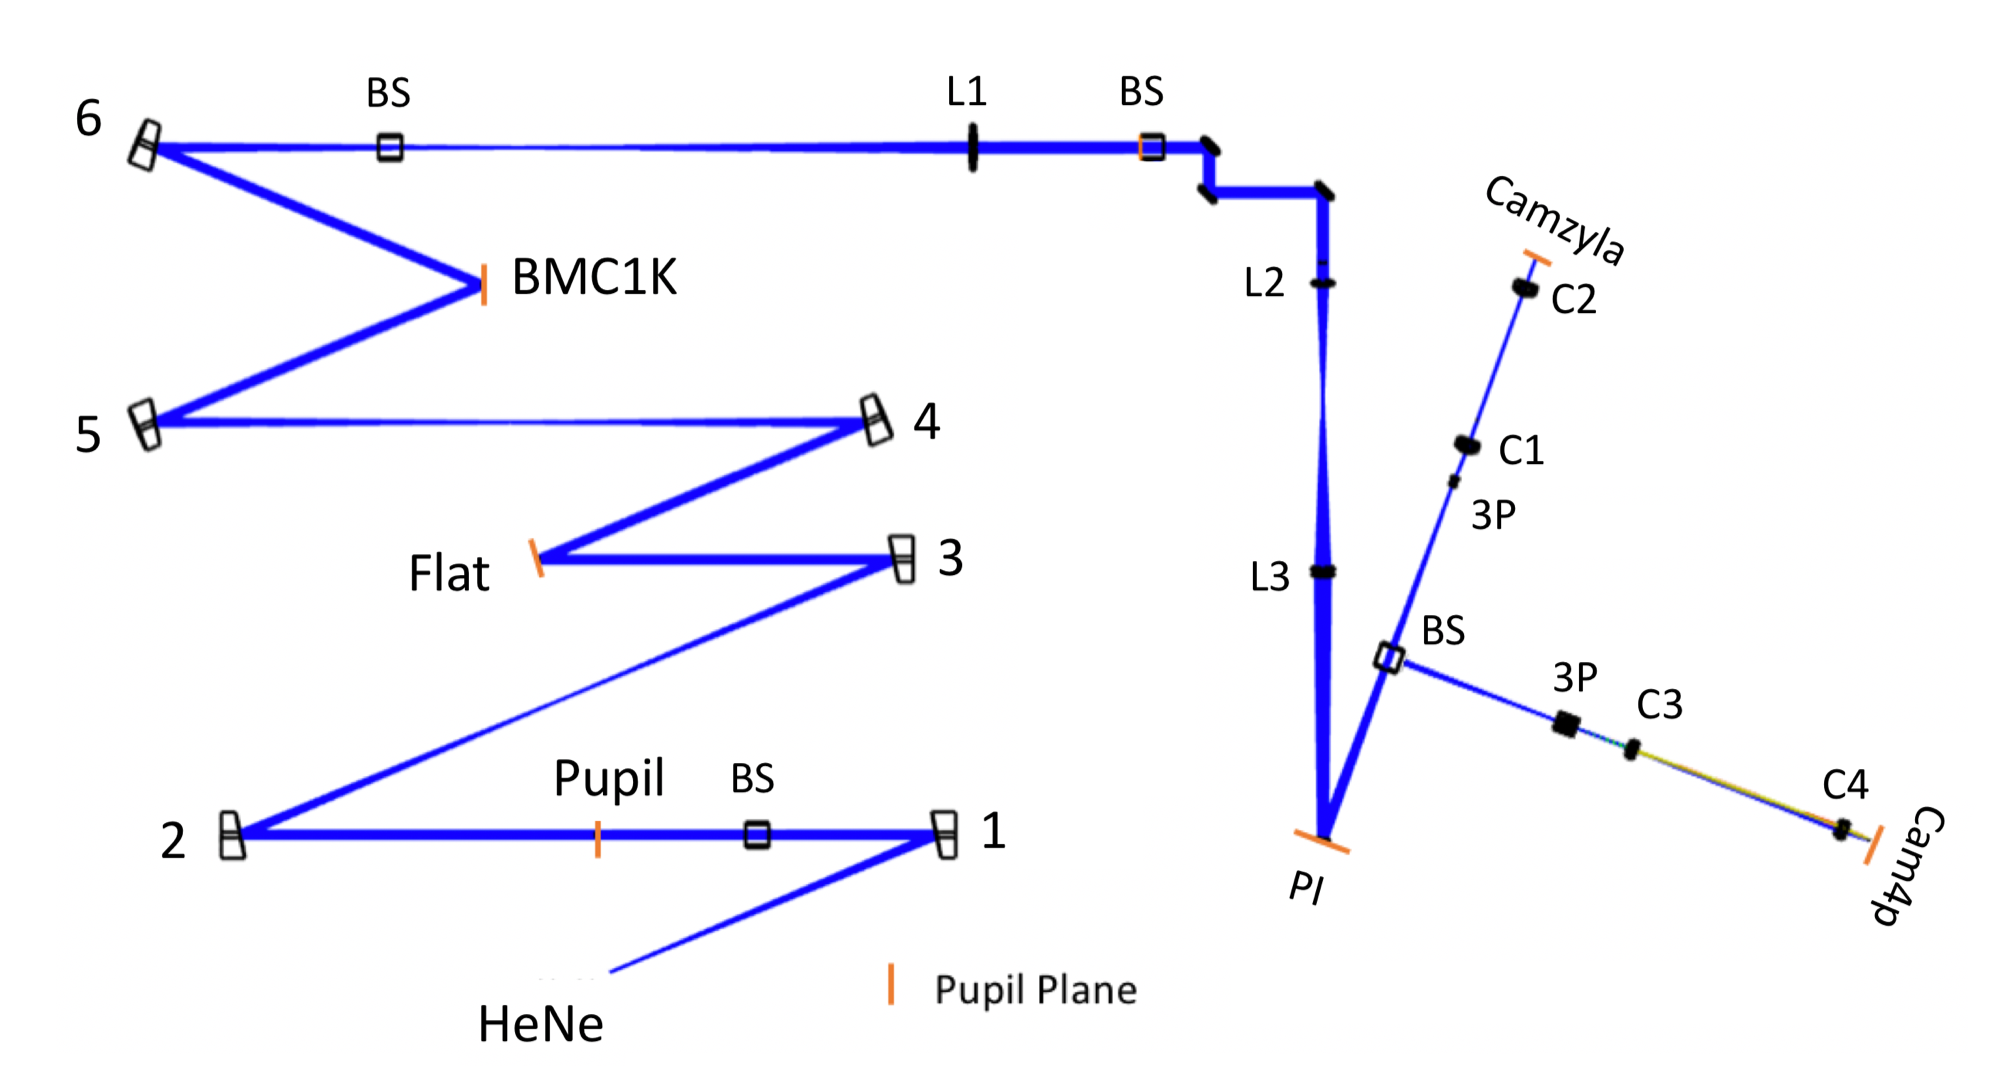
\includegraphics[width=0.8\textwidth]{Chapter Materials/Chapter Five Materials/CACTIzemax.png}
    \caption{Optical design of CACTI. Light starts from a point source from the HeNe laser and relayed through a series of afocal pupil relays. The focal plane of the AO simulator is after the 6${^{th}}$ OAP. It is collimated by a lens and passed into the PWFS testbed. A beamsplitter sends the same focal plane to both the 3PWFS and 4PWFS to minimize non-common path errors.}
    \label{fig:CACTIZemax}
\end{figure}

CACTI was designed to simulate atmospheric turbulence in a complete closed loop AO system. The optical design of  CACTI  is shown in Figure \ref{fig:CACTIZemax} and Table \ref{tab:CACTItable} summarizes the main components. The layout on the optical table is shown in Figure \ref{fig:CACTI}. A Helium-Neon (HeNe) laser (wavelength 633-$nm$) is used for inital alignment and testing.  The light is passed to a spatial filter with a 10-$\mu m$ pinhole to clean up any wavefront errors, and insure that the start of the system is an unresolved point source. The point source is then collimated by an off-axis parabolic (OAP) mirror to simulate starlight coming from infinity. There are six OAP mirrors in total that form the pupil relays of the system. All are cored from the same parent with $\lambda /10$ surface quality (Peak-to-Valley). Each OAP has a focal length of 375.25-$mm$ and an off-axis angle of 23 degrees. A 50/50 beamsplitter cube is placed into the collimated beam after the first OAP as an optional input for another collimated light source. After the beamsplitter a 7.5-$mm$ in diameter circular clear aperture mask is placed to define the entrance pupil of CACTI. The first pupil relay formed by the 2$^{nd}$ and 3$^{rd}$ OAP mirrors re-images the entrance pupil onto a flat mirror that is mounted on a kinematic base. The flat mirror is intended to be removed and replaced by a DM in the future. The second pupil relay created by the 4$^{th}$ and 5$^{th}$ OAP mirrors, relays the pupil onto a 1024 actuator Boston Micromachine 1K (BMC1K) DM. In the experiments described here, the BMC1K is used to simulate the atmosphere, correct the errors in closed-loop with the wavefront sensor, and correct for common path errors from misalignments. The last OAP focuses the light to the final focal plane in the AO simulator. A 50/50 beamsplitter is placed in this converging beam so that an additional focal plane can be accessed. In the current configuration of CACTI we have placed a Basler ACE CMOS camera as our science camera (Camsci) at this focal plane.


\begin{table}
	\begin{center}
		\begin{tabular}{ | l| l | }
			\hline
			\textbf{Component}& \textbf{Description}\\ \hline
			Light Source & Helium-Neon laser 633-$nm$ $\lambda$\\ \hline
			Spatial filter & 10-$\mu m$ Pinhole \\ \hline
			Off-axis parabolic mirrors & 375.25-mm Focal length, 23$^{\circ}$ off-axis angle \\ \hline
            Entrance pupil & 7.5-mm Clear aperture mask \\ \hline
            Deformable mirror & Boston Micromachines, 1024 Actuator, 9mm in diameter \\ \hline
            Beamsplitters & 50/50 Cube beamsplitter \\ \hline
            Modulation Mirror &  PI S-331 Piezo-actuator stage \\ \hline
            3PWFS Optic & Fused silica glass monolith \\ \hline
            4PWFS Optic & Crossed roof prisms \\ \hline
            Science Camera (Camsci) & Basler ACE acA640-750um CMOS\\ \hline
            3PWFS Camera (Camzyla) & Zyla 4.2+ sCMOS detector \\ \hline
            4PWFS Camera (Cam4p) & Basler ace acA720-520um CMOS \\ \hline
            Lens 1 (L1) & Doublet 500-mm focal length  \\ \hline
            Lens 2 (L2) & Doublet (CHECK ZEMAX)  \\ \hline
            Lens 3 (L3) & Custom achromatic air-spaced triplet  \\ \hline
            3PWFS Camera lens 1 (C1) & Doublet 30-mm focal length \\ \hline
            3PWFS Camera lens 2 (C2) & Doublet 30-mm focal length \\ \hline
            4PWFS Camera lens 1 (C3) & Doublet 50-mm focal length \\ \hline
            4PWFS Camera lens 2 (C4) & Doublet 30-mm focal length \\ \hline
				
			\end{tabular}
		\end{center}
	\caption{Descriptions of the components in CACTI.}
	\label{tab:CACTItable}
\end{table}

\begin{figure}
    \centering
    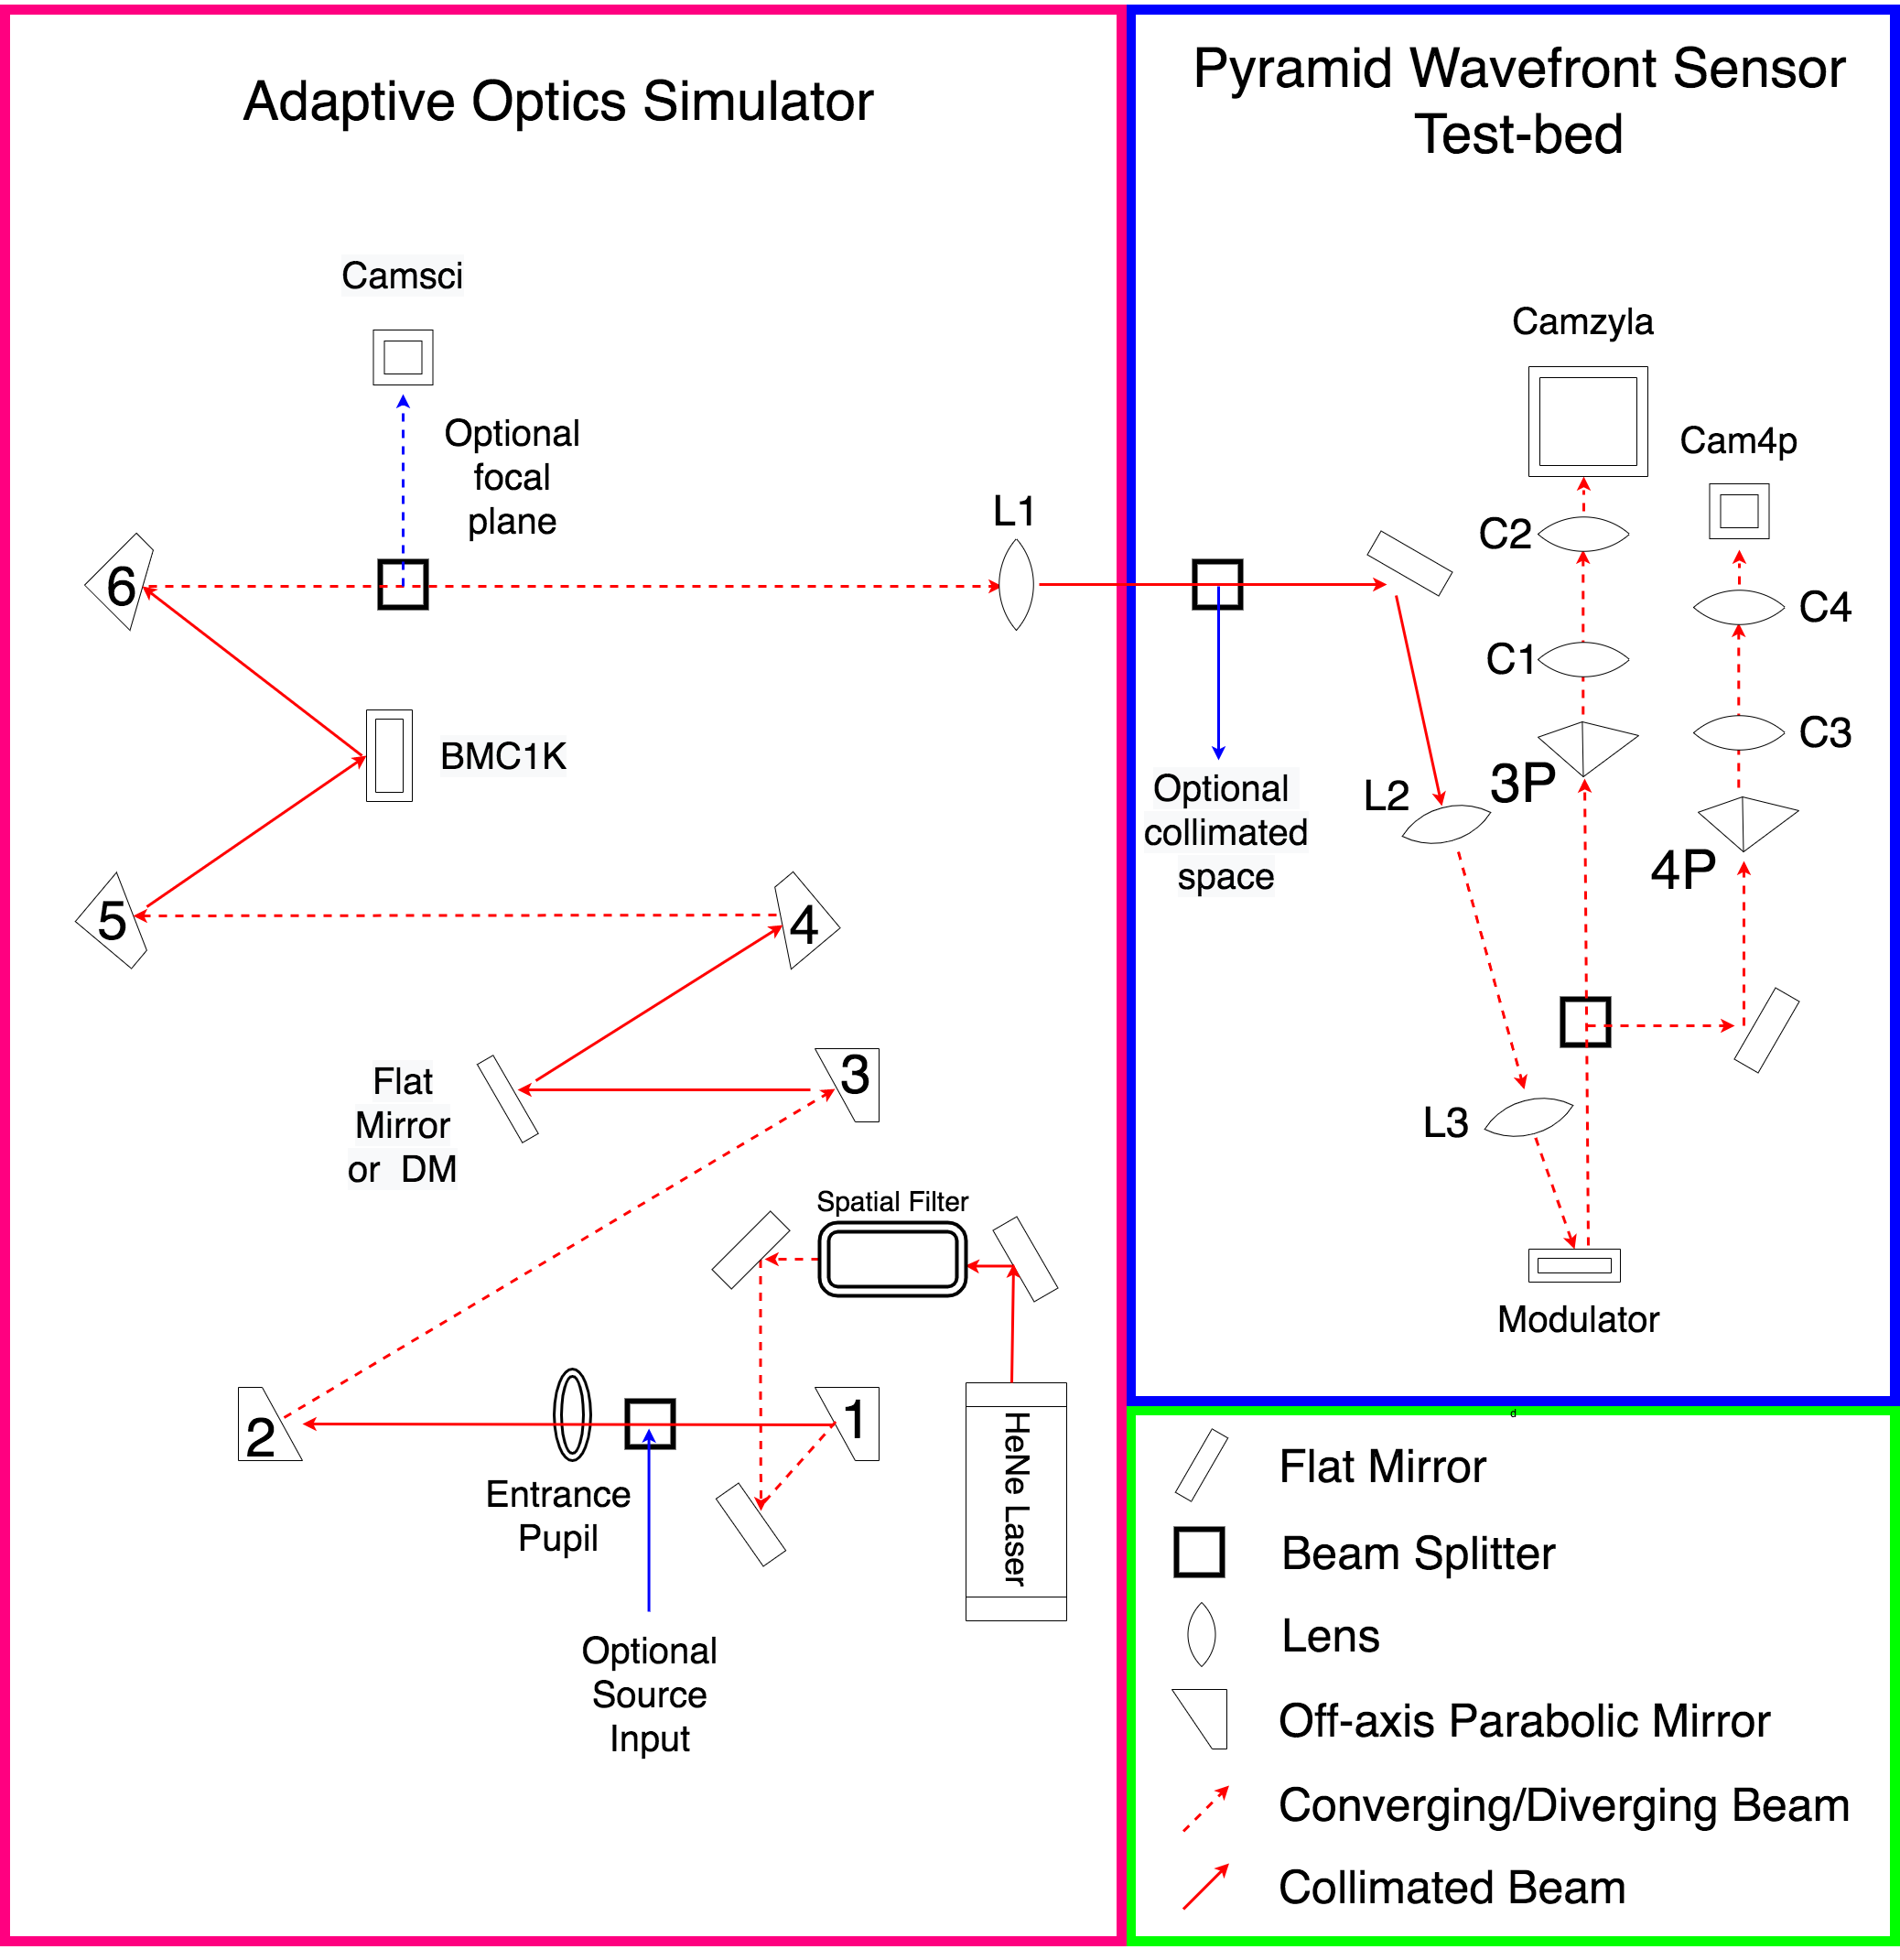
\includegraphics[width=0.8\textwidth]{Chapter Materials/Chapter Five Materials/CACTI.png}
    \caption{In the current configuration CACTI consists of an Adaptive Optics Simulator and the PWFS testbed. Beamsplitters are used in CACTI to provide access to focal planes, collimated spaces, and additional sources. In the current configuration light is relayed through the AO simulator onto the 1024 actuator Boston Micromachine 1K (BMC1K) DM OAP mirrors. The light is then passed to the PWFS testbed which includes a modulation mirror, a 4PWFS and a 3PWFS.}
    \label{fig:CACTI}
\end{figure}

\subsection{Software and Calibration}

CACTI uses the Compute And Control For Adaptive Optics (CACAO) real-time control software package \citep{guyon2018compute}. The calibration of the AO system by CACAO is a multi-step process. Hadamard modes are applied to the DM, and the WFS response is recorded. The WFS signals from the Hadamard modes are then decomposed into the response of the influence functions from single actuators. These influence functions are then projected onto Fourier modes to create the basis set for the modal wavefront control. In these steps the illumination pattern of the deformable mirror is determined by thresholding actuators that don't give a response in the wavefront sensor. Similarly a mask of the PWFS detector pixels is generated to keep only the valid pixels from the PWFS pupils on the detector that will be used for wavefront sensing. CACAO is also used to generate the phase screens to simulate turbulence. Due to the limited low-order stroke of the BMC1K, the power-spectrum of the turbulence generated by CACAO is filtered to suppress the low order modes so that the full stroke of the DM is not used. At middle to high spatial frequencies the power spectrum matches that of Kolmogorov turbulence. 



%%%%%%%%%%%%%%%%%%%%%%%%%%%%%%%%%%%%%%%%%

\subsection{Designing OAPs in Zemax}
The main design effort for the AO simulator was modeling the OAP mirrors. The OAP mirrors on CACTI were cored from a parent parabolic mirror. Each OAP has the same focal length and off-axis angle. The off-axis angle of an OAP mirror is determined by the distance to the axis of the parent mirror. OAPs that are cored close to the edge of the parent mirror have large off-axis angles, and a significant wedge. Figure \ref{fig:OAPedmund} is a picture of an OAP mirror with a 90$^{\circ}$ off-axis angle and a significant wedge \citep{edmundoptic}. The wedge of the OAP mirror is helpful for incorporating OAP mirrors into a design, because the wedge informs the clocking of the OAP in the mirror mount, and the tilt of the OAP with respect to the optical table. The bottom edge of the thick portion of the wedge should be parallel with the collimated beam. Figure \ref{fig:OAPcol} is a Zemax model of an OAP collimating a point source. The OAP is rotated and clocked so that the bottom edge of the thick wedge is parallel to the collimated beam. 

\begin{figure}
    \centering
    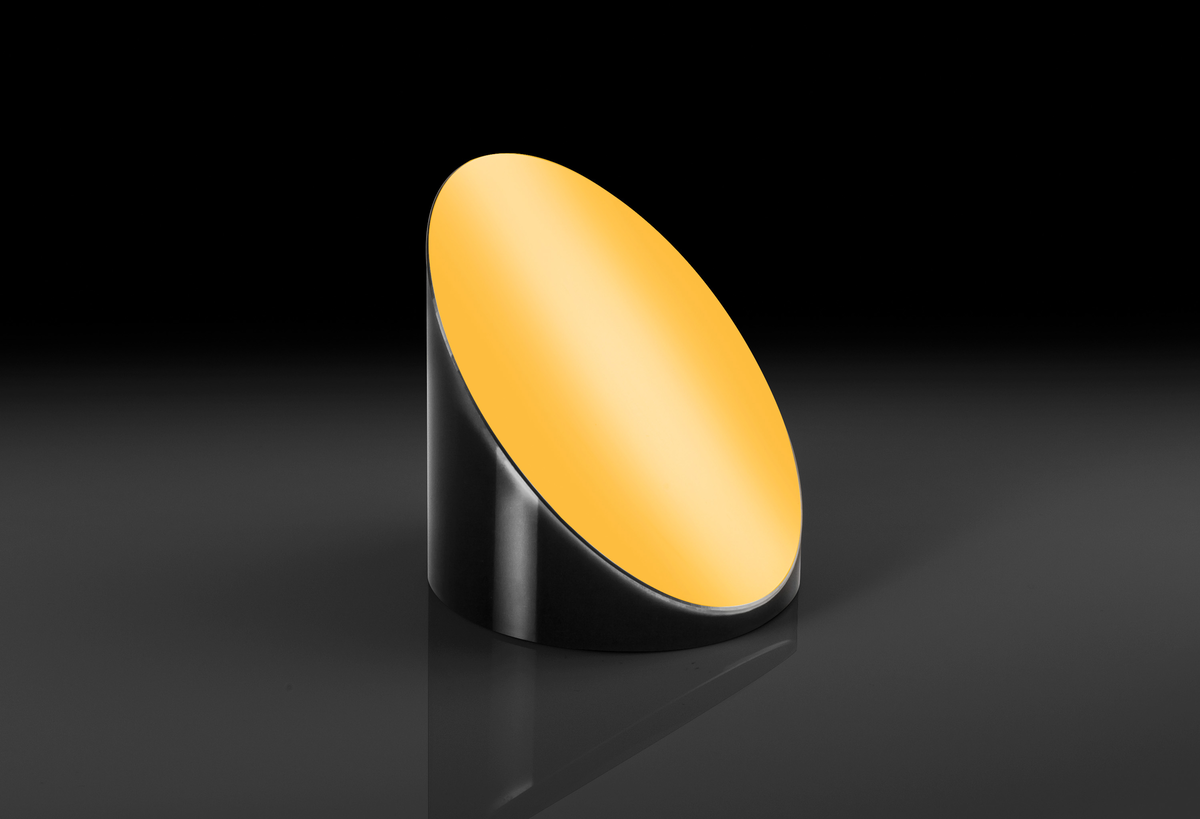
\includegraphics[width=0.8\textwidth]{Chapter Materials/Chapter Five Materials/OAP.png}
    \caption{Image of an OAP mirror with a 90$^{\circ}$ off-axis angle \citep{edmundoptic}.}
    \label{fig:OAPedmund}
\end{figure}


\begin{figure}
    \centering
    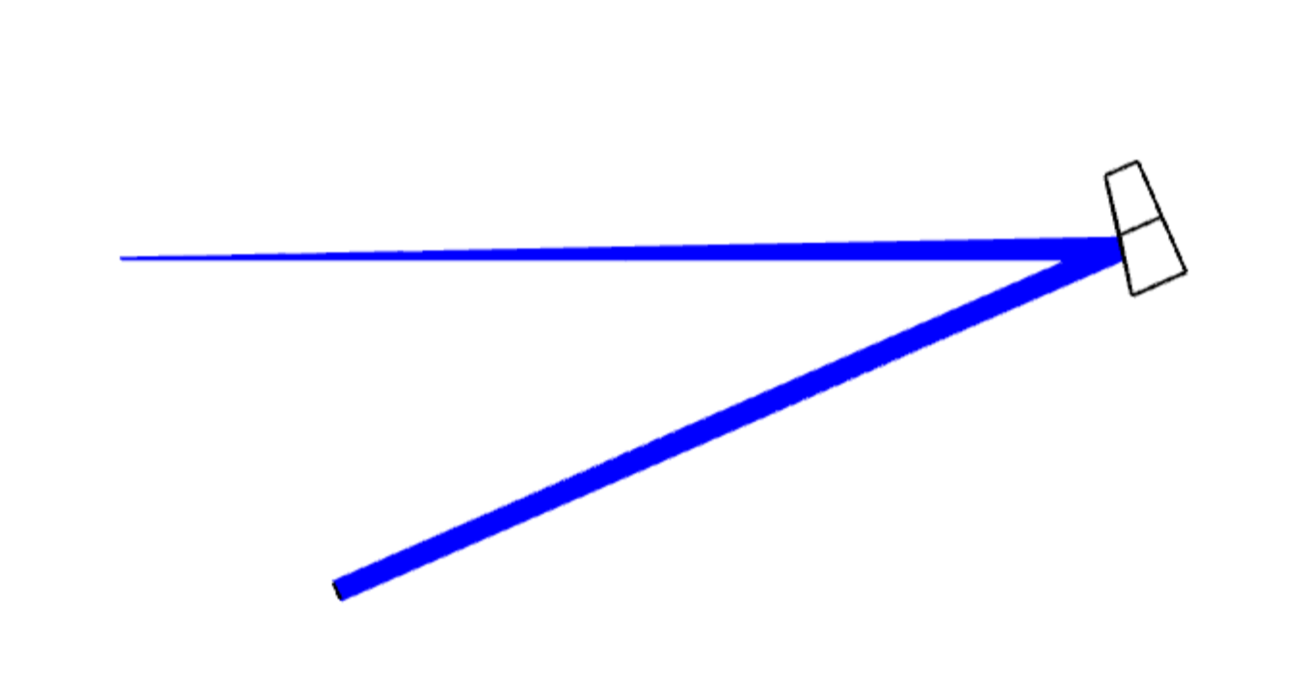
\includegraphics[width=0.8\textwidth]{Chapter Materials/Chapter Five Materials/OAPcollimate.png}
    \caption{Zemax diagram of a point source collimated by an OAP mirror. The thick bottom edge of the OAP wedge is always parallel to the collimated beam. }
    \label{fig:OAPcol}
\end{figure}

OAPs are modeled in Zemax by designing a parabolic mirror and decentering it with respect to the optical axis. The clocking of the OAP is determined by how the parabolic mirror is decentered. For example in Figure \ref{fig:OAPex} the parent parabola is shifted below the optical axis of the system. This results in the illumination of the top portion of the parabolic mirror, which has a wedge shape where the thickest part of the wedge is on top. If the inverse of that wedge was needed, the parent parabola would be shifted above the optical axis of the system. 

\begin{figure}
    \centering
    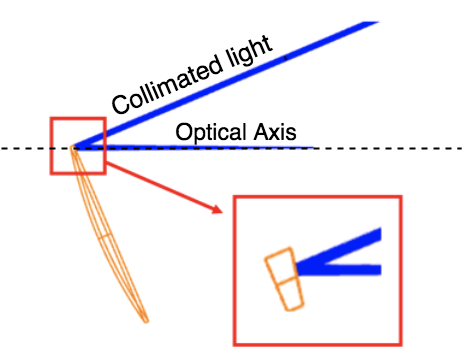
\includegraphics[width=0.8\textwidth]{Chapter Materials/Chapter Five Materials/OAPexample.png}
    \caption{Diagram of how OAP mirrors are modeled in Zemax. A parabolic mirror is shifted and tilted to achieve the effect of an OAP mirror.}
    \label{fig:OAPex}
\end{figure}

Using this knowledge of OAP design we can set solves in the Zemax design to correctly place OAPs. In the lens data editor a coordinate break around the OAP. The Decenter-Y value before the mirror surface is set to be variable, and the Decenter-Y value after the mirror is set to a chief ray solve. The tilt of the OAP can be adjusted by changing the tilt-about-X variable.  In the merit function set operands to minimize the RMS wavefront error and to insure that the rays leaving the mirror are parallel to the optical axis if the OAP is being used to collimate. If done correctly the optimization will set the parabolic mirror at the correct decenter and create a perfectly collimated beam from a point source. In zemax the distances between optics is displayed at the thickness variable in the lens data editor. Zemax calculates that distance based on the vertex of the mirror, which for OAPs is the vertex of the parent parabola. To find the correct distances between OAP mirror surface use operands in the merit function to determine the vertices of the mirror surfaces and solve for the distances between them using math operands. 



\subsection{Pyramid Wavefront Sensor Testbed}

ExAO systems need high sampling of the wavefront to optimize performance, and as a result, require larger detectors. An ideal wavefront sensing camera for ExAO has a large number of pixels that can be read out at a fast speed with low read noise. In choosing detectors, there is a trade-off between detector, size, speed and noise. We are interested in exploring the 3PWFS as an alternative wavefront sensor for the GSMTs because the 3PWFS uses fewer detector pixels than the 4PWFS. Previous work has shown in simulation that the 3PWFS is less sensitive to read noise, resulting in a modest boost in performance, (Schatz et al, 2021 in review). The goal of this study is to test a 3PWFS using CACTI, and expand the previous study to understand how the 3PWFS performs under different turbulence conditions compared to the 4PWFS. 

The design of the PWFS testbed is detailed in Figure \ref{fig:CACTI}. Light from the AO simulator is collimated by a 500-mm focal length lens (L1) which relays the exit pupil of the AO simulator to the PWFS testbed. The exit pupil of the AO simulator becomes the entrance pupil to the PWFS testbed, which is then resized by a pupil relay consisting of an achromatic doublet (L2) and a custom air-spaced achromatic triplet lens (L3). The pupil is imaged on the the modulation mirror, which is a $\lambda/20$ flat mirror mounted on a PI S-331 high speed piezo-actuator tip/tilt platform. A 3PWFS designed by Hartsci LLC has been integrated into the instrument for the performance test. The three sided pyramid optic is single prism made from fused silica glass and has a tip smaller than 5 microns that was custom made for this experiment. Figure \ref{fig:pyramidOptics}.A shows the 3D model of the manufactured prism. The 4PWFS in CACTI uses two crossed roof prisms for its pyramid optic shown in Figure \ref{fig:pyramidOptics}.B. This is the same type of pyramid used in the SCExAO \citep{jovanovic2015subaru}.  A 50/50 beamsplitter after the modulation mirror sends the same PSF to the pyramid tips of the 3PWFS and 4PWFS to mitigate non-common path errors, as all the optics up to that point are common to both wavefront sensors. The PSF on the pyramid tips were sharpened by the DM using a grid search that applies different amplitudes of Zernike modes on the deformable mirror, and saves the combination of modes that maximizes the Strehl Ratio at the focal plane as the  DM set point where non-common path errors are minimized, (K. Van Gorkom et al. (2021, submitted)).

\begin{figure}
    \centering
    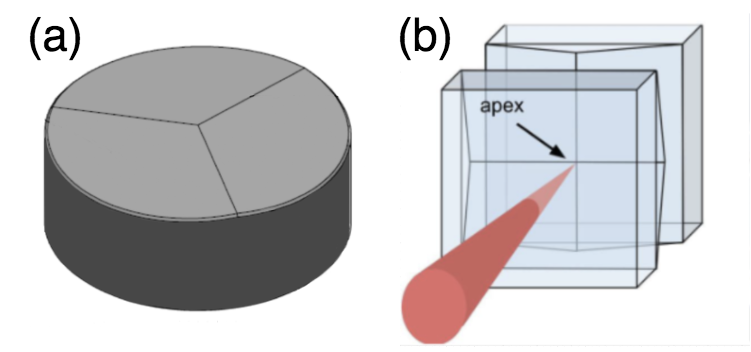
\includegraphics[width=0.8\textwidth]{Chapter Materials/Chapter Five Materials/pyramidOptics.png}
    \caption{Drawings of the pyramid optics in CACTI. A. The 3PWFS pyramid is a single prism made from fused silica glass. The 4PWFS pyramid is two crossed roof prisms. This pyramid is a copy of of the pyramid used by SCeXAO \citep{jovanovic2015subaru}. }
    \label{fig:pyramidOptics}
\end{figure}


The pupil of each PWFS are imaged on the the detectors by using two camera lenses, C1 and C2 for the 3PWFS, and C3 and C4 for the 4PWFS,  that form a zoom lens system to insure that the sizes of pupils from both PWFS are 30 pixels in diameter. The 3PWFS uses a Andor Zyla 4.2+ sCMOS and the 4PWFS uses a Basler ace acA720-520um CMOS camera. Schatz et al. found in simulation that when the PWFS are well illuminated by light the effects of read noise to performance are negligible. The experiments performed in this paper were under bright light conditions, so having different cameras with different noise characteristics should not effect the PWFS performance. The average count per pixel for a 3PWFS pupil was 1188 counts determined by calculating the average pixel value for only the pixels within the pupils over 1000 frames with a flat applied to the DM. The PWFS signals on CACTI can be processed in two ways, the Raw Intensity (RI) and Slopes Maps (SM) methods. In both methods the detector signal from the PWFS is dark subtracted, and a threshold is applied to mask out any pixels outside of the PWFS pupils. In the RI method the remaining signal is used as-is. The Slopes Maps calculation recombines the PWFS pupils into an estimate of the X and Y slopes of the wavefront slope. The SM equation for the 4PWFS is given in Equation \ref{4PWFSslopes}, and the Equation for the 3PWFS is given in \ref{3PWFSslopes}. In these equations $S_x, S_y$ are the local wavefront slopes, and $I_1...I_4$ are the intensity values of the pixel corresponding to the same location in each pupil.


\begin{eqnarray}
    S_x=\frac{I_1+I_2-I_3-I_4}{I_1+I_2+I_3+I_4}     \label{4PWFSslopes} \\
    S_y=\frac{I_1-I_2-I_3+I_4}{I_1+I_2+I_3+I_4} \nonumber
\end{eqnarray}

\begin{eqnarray}
    S_x=\frac{\frac{\sqrt{3}}{2}I_2-\frac{\sqrt{3}}{2}I_3}{I_1+I_2+I_3} \label{3PWFSslopes} \\
    S_y=\frac{I_1-\frac{1}{2}I_2-\frac{1}{2}I_3}{I_1+I_2+I_3} \nonumber
\end{eqnarray}


\subsection{Designing Pyramid Optics in Zemax}

For the CACTI testbed the pyramid optics were designed using sequential ray tracing. The pyramid optic was modeled as a plate of glass that is tilted to mimic that angle of the pyramid facets. Multiple configurations were used to rotate the plate to create the facets of the pyramid and trace rays at different locations to create the focal plane splitting. The sizes and separations of the pupils were set by setting the distances between the camera lenses, the PWFS, and the science camera as variable. Each lens was first modeled as a paraxial lens, and the focal length was set to variable. After a first iteration of design real lenses were chosen with similar focal lengths and incorporated into the model. The merit function was defined to minimizes aberrations in the system and set the sizes and separations of the pyramid pupils to our requirements. The resulting pupils can be viewed in the beam footprint diagram. It was necessary to create a dummy surface before the image and set the reference coordinate system to that surface so that Zemax displays the pupils of each configuration correctly. If left in the normal configuration, Zemax will display the pupils as overlapping, because each pupil will be plotted with respect to its own coordinate system and not the global coordinate system. The beam footprint for the 3PWFS and 4PWFS are given in Figure \ref{fig:beamfp}.A and Figure\ref{fig:beamfp}.B. 

\begin{figure}
    \centering
    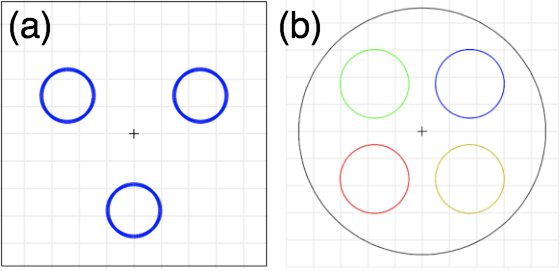
\includegraphics[width=0.8\textwidth]{Chapter Materials/Chapter Five Materials/BeamFootPrint.png}
    \caption{Beam foot prints of the PWFS pupils from a 3PWFS and 4PWFS modeled in Zemax. A. Is the beam footprint from the 3PWFS. B. Is the beam footprint from the 4PWFS.  }
    \label{fig:beamfp}
\end{figure}


\subsection{Current Status}

The alignment of the adaptive optics simulator and PWFS tesbed in CACTI was completed in May 2020. Figure \ref{fig:cactiTestbed} is a picture of the as built system. Light from the HeNe laser is relayed by the six OAP mirrors, and is then coupled to the PWFS testbed using a beam triangle formed by two flat mirrors. Figure \ref{fig:PWFStestbed} is a close up diagram of the PWFS testbed. The first two lenses (L1 and L2) relay the entrance pupil of the PWFS testbed onto the PI modulation mirror (PI). A beamsplitter after the modulation mirror picks off light to the four-sided pyramid (4P) and the through beam is sent to the three-sided pyramid (3P). Both pyramids have two camera lenses (C1 and C2) that form a zoom lens to match the diameters of the pupils of the two PWFS. The measured pupil diameter for the 4PWFS is 30.5 pixels and 29.5 pixels for the 3PWFS. 

\begin{figure}
    \centering
    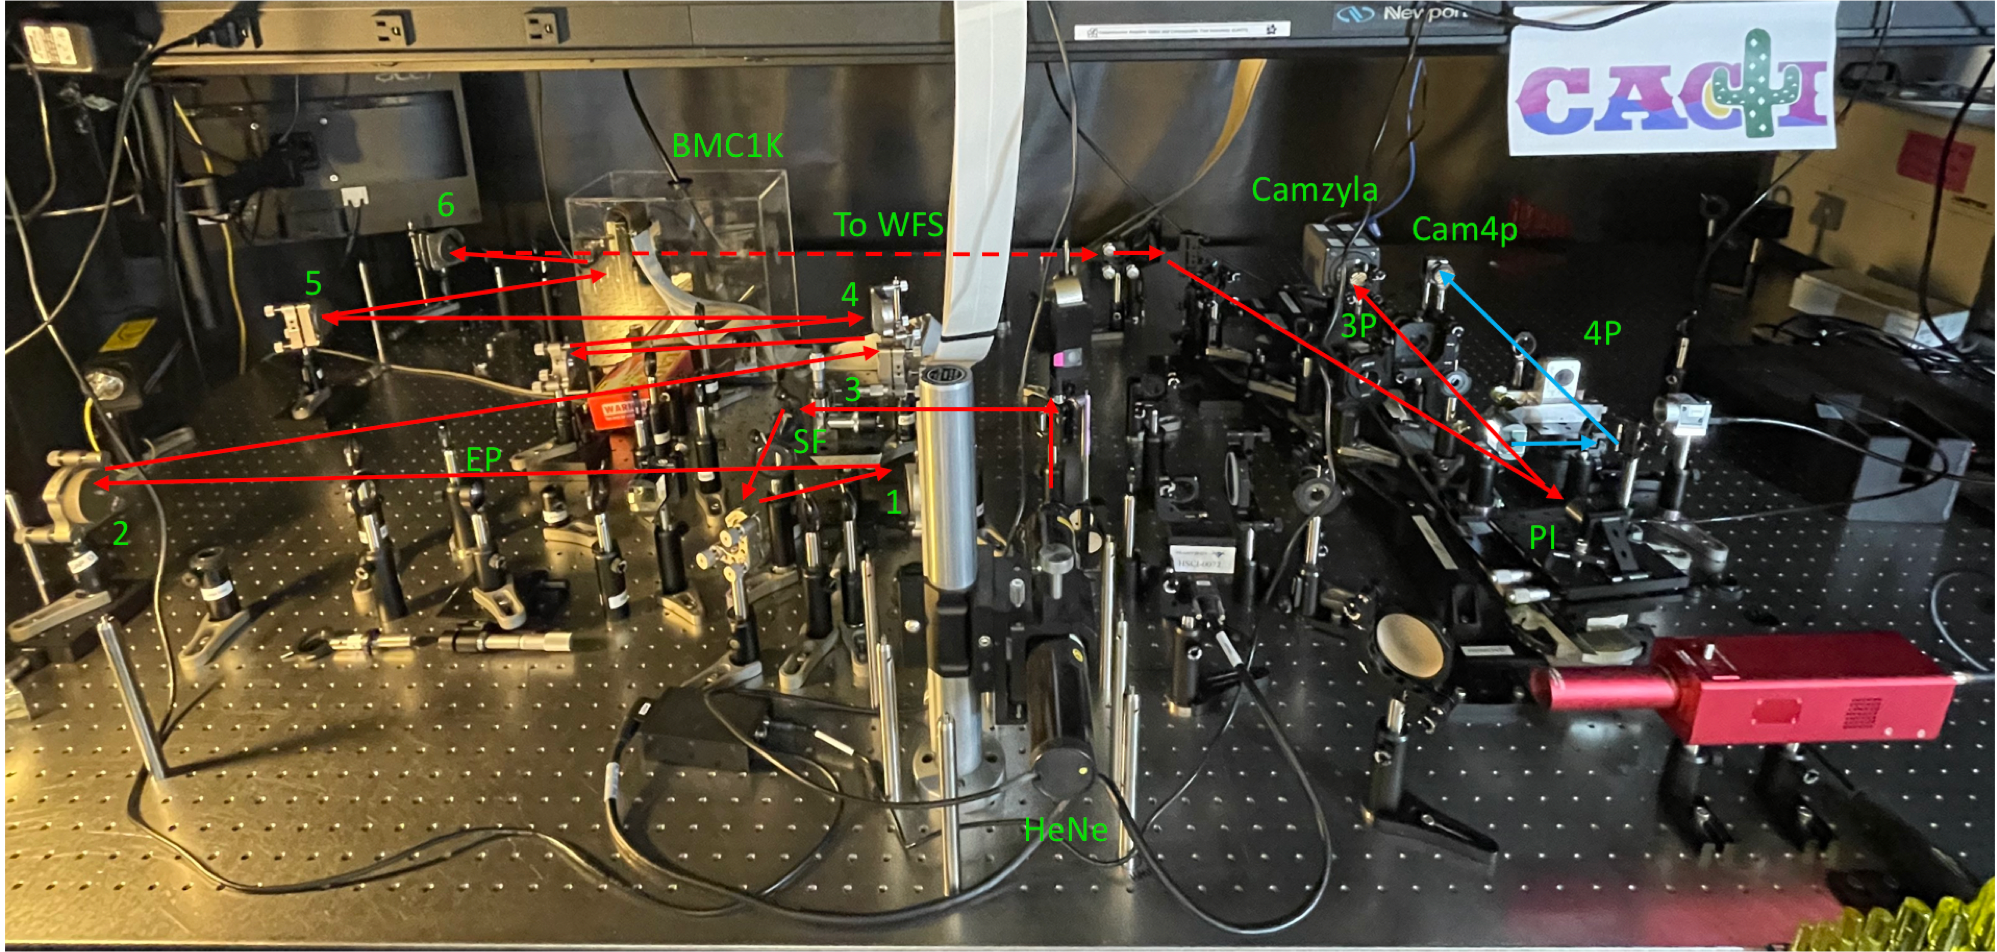
\includegraphics[width=0.8\textwidth]{Chapter Materials/Chapter Five Materials/cactiTestbed.png}
    \caption{Image of the as-built CACTI testbed. Light starts from the HeNe laser and propagates through the AO simulator on the left half of the optical table. After the BMC1K and the final OAP, the light is relayed to the PWFS testbed on the right half of the optical table.}
    \label{fig:cactiTestbed}
\end{figure}

\begin{figure}
    \centering
    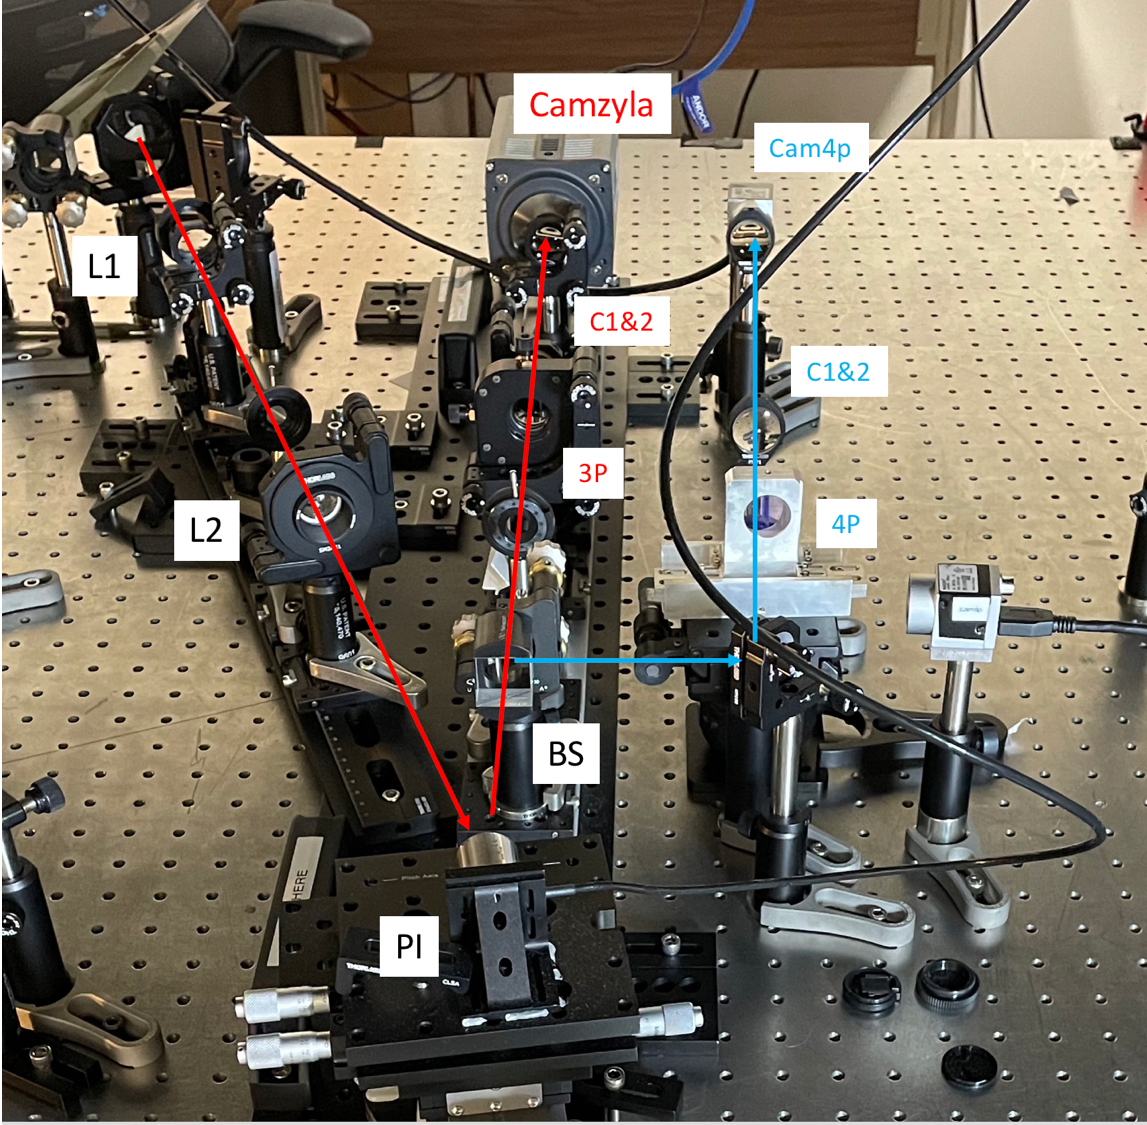
\includegraphics[width=0.8\textwidth]{Chapter Materials/Chapter Five Materials/PWFStestbed.png}
    \caption{Close up image of the PWFS testbed. Light enters the system before L1 on the left side. The light is relayed onto the modulation mirror (PI). The through beam propagates through to the 3PWFS which consists of the pyramid optic (3P), camera lenses (C1$\&$2) and the Zyla CMOS camera (Camzyla). Light is by a beamsplitter (BS) to the 4PWFS arm which consists of the pyramid (4P), camera lenses (C3$\&$4) and the Basler CMOS camera (Cam4p).  }
    \label{fig:PWFStestbed}
\end{figure}


 The system responses to the flat wavefront generated by the deformable mirror is given by Figure \ref{fig:flatCACTI}. Figure \ref{fig:flatCACTI}.A is the PSF in logarithmic scale on our science camera. Figure \ref{fig:flatCACTI}.B similarly is the PSF on the pyramid tip also in log scale. Figure  \ref{fig:flatCACTI}.C and Figure \ref{fig:flatCACTI}.D are the pyramid pupils from a flat wavefront with 5$\lambda/D$ modulation for the 3PWFS and 4PWFS respectively. There is a ghost in the CACTI PWFS located at the 4$^{th}$ Airy ring and caused by one of the lenses in the system. 

\begin{figure}
    \centering
    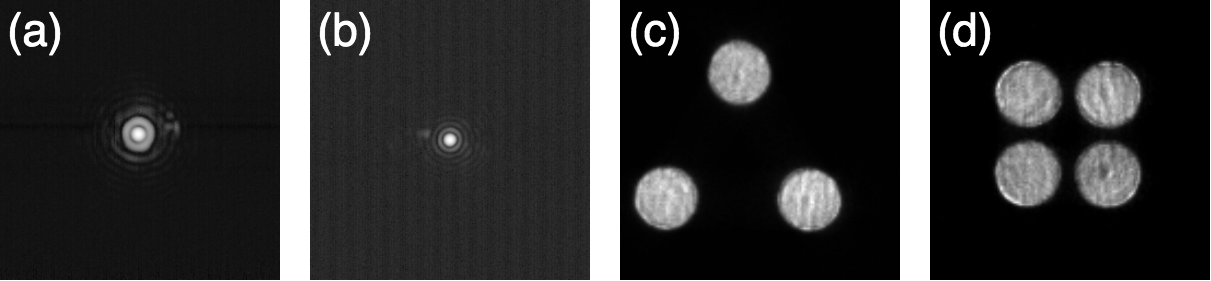
\includegraphics[width=0.8\textwidth]{Chapter Materials/Chapter Five Materials/flatCACTI.png}
    \caption{Signals from CACTI in response to the optimized flat wavefront. A. The PSF on the science camera. B. The optimized PSF on the focal plane of the PWFS tips. C. The 3PWFS pupils on Camzyla at 5 $\lambda/D$ modulation. D. The 4PWFS pupils on Cam4p at 5 $\lambda/D$ modulation.}
    \label{fig:flatCACTI}
\end{figure}


We have successfully closed the AO loop on CACTI with both the 4PWFS and 3PWFS using both the RI and SM signal handling methods. This marks the first time the AO loop has been closed on a glass pyramid 3PWFS. Previous work by Schatz et al. closed the AO loop on a 3PWFS on the LOOPS testbed at the Laboratoire d'Astrophysique de Marseille, created by a phase screen applied to a spatial light modulator. 


The deformable mirror on CACTI was used to both generate the turbulence screen and apply the correction. This is done using the CACAO software which creates multiple channels of commands for the deformable mirror. In one channel we can stream the turbulence phase screens, and in another channel we have the commands computed by real time control software using the PWFS signals. The actual command applied to the DM is a summation of commands from all of the channels. Figure \ref{fig:turbCACTI} shows the closed loop PSFs and pyramid pupils from a turbulence strength of 0.3-$\mu m$ RMS error on CACTI. Figure \ref{fig:turbCACTI}.A and \ref{fig:turbCACTI}.B are the 3PWFS pupils and the closed loop PSF in log scale on the science camera. Figure \ref{fig:turbCACTI}.C and \ref{fig:turbCACTI}.D are the 4PWFS pupils and the closed loop PSF in log scale on the science camera.

% \jrmcom{GREAT STUFF!!!}

\begin{figure}
    \centering
    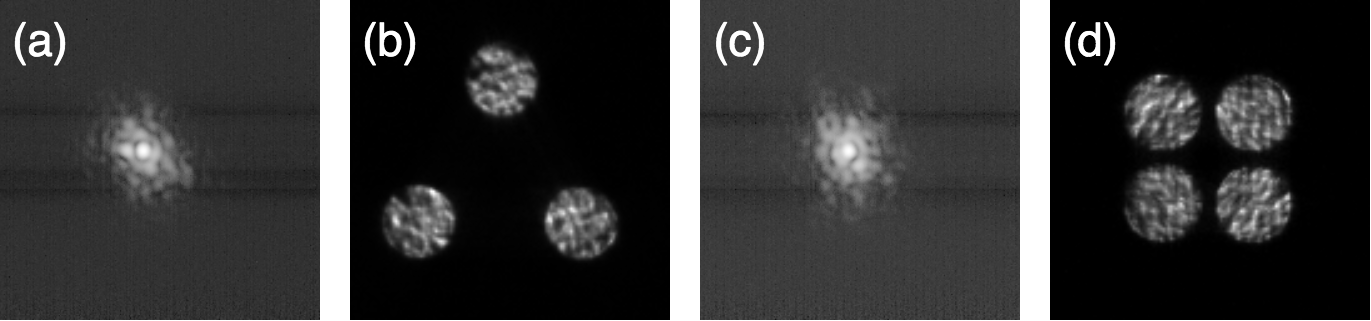
\includegraphics[width=0.8\textwidth]{Chapter Materials/Chapter Five Materials/turbCACTI.png}
    \caption{A. Time-averaged science camera image of the 3PWFS closed-loop PSF in log scale. B. Turbulence streaming across the 3PWFS pupils. C. Time-averaged science camera image of the 3PWFS closed-loop PSF in log scale. D. Turbulence streaming across the 4PWFS pupils.}
    \label{fig:turbCACTI}
\end{figure}


\section{Experimental Details}


The CACTI testbed was used to compare the performance of a 3PWFS and 4PWFS in varying strengths of turbulence. Previous work by Schatz et al. found in simulation that the performance of the two wavefront sensors are comparable. These simulations however were run for only one seeing condition. The goal of this experiment is to determine the relative performance of the 3PWFS to the 4PWFS in varying strengths of turbulence using both the Raw Intensity and Slope Maps signal processing methods. The performance was determined by measuring the relative Strehl ratio of the AO corrected PSF and the aberration free PSF. For the CACTI testbed our aberration free PSF was the flat wavefront PSF on the science camera created by the deformable mirror shown in Figure \ref{fig:flatCACTI}.A., which we will refer to as the reference PSF. The reference PSF was used in the calibration of each PWFS. To calculate the Strehl Ratio we developed a Strehl Calculation pipeline detailed in Appendix A.

The experiment performed on CACTI was to measure the Strehl Ratio as a function of turbulence strength and modulation radius for both the 3PWFS and the 4PWFS.  This experiment was performed using the Raw Intensity signal handling method. The modulation radii used were: 1.6 $\lambda/D$, and 3.25 $\lambda/D$. At each modulation radius the following experiment was performed at a loop speed of 400-Hz:

\begin{itemize}
    \item Apply the best flat commands on the DM and create the reference PSF from the average of 1000 frames.
    \item Dark frames taken for each of the cameras and subtracted from each PWFS frame as a signal processing step in the closed loop. Dark frames created from an average of 1000 frames
    \item A new calibration to generate a reconstructor matrix was taken for each modulation radius.
    \item Apply simulated turbulence at levels 0.1-$\mu m$, 0.2-$\mu m$, 0.3-$\mu m$, 0.4-$\mu m$, 0.5-$\mu m$, and 0.6-$\mu m$, RMS wavefront error. 
    \item At each phase screen record 50 closed-loop PSF images, where each image is created from taking the average from 300 frames of data. 
    \item Calculate the average Strehl value from the closed-loop PSFs to create an average Strehl value for each turbulence strength.
    \item Plot the Strehl value as a function of turbulence strength and magnitude radius. 
    
\end{itemize}

The loop gain for the experiments was set to 0.8. CACAO allows for gains to be set for blocks of spatial frequencies. For example modal block 00 controls the gain of Tip/Tilt and block 01 controls Focus. The modal gains were optimized for each PWFS configuration by performing a crude search. At high levels of turbulence the modal gains were tuned to maximize the AO system correction by eye. PSF frames were recorded and a Strehl ratio was calculated for those values of gains. The gains were then adjusted and the same procedure was performed until the values of the modal gains converged to give a good correction. Figure \ref{fig:gains} plots the modal loop gain value against the modal frequency block number.

\begin{figure}
    \centering
    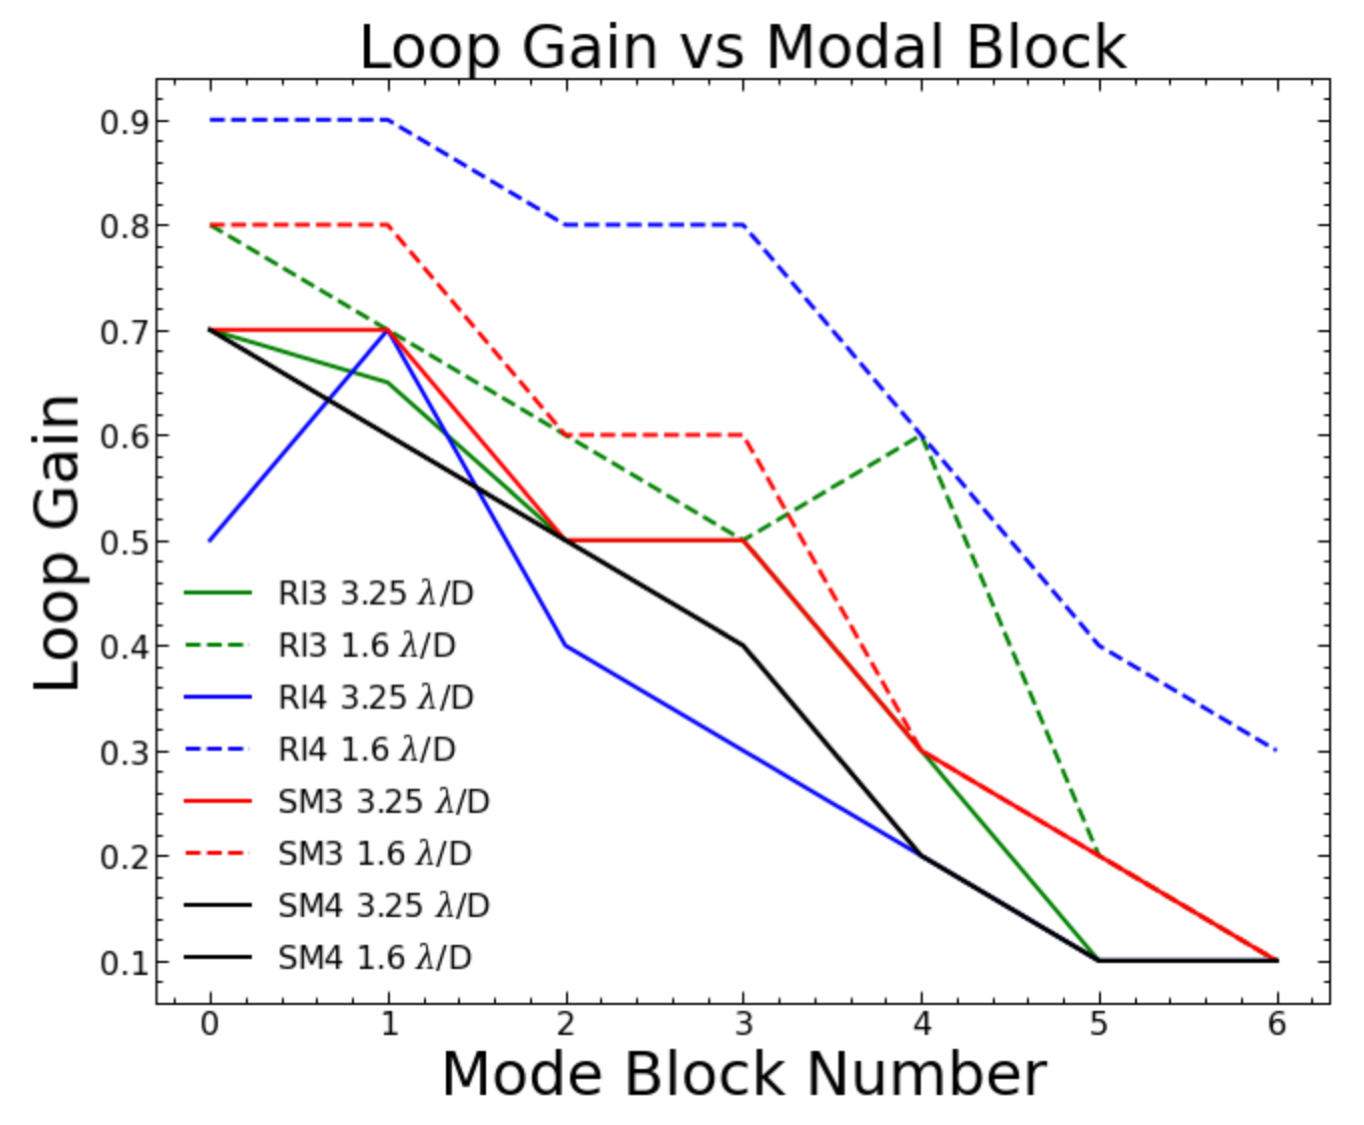
\includegraphics[width=0.6\textwidth]{Chapter Materials/Chapter Five Materials/ModeVsLoopGain.png}
    \caption{Loop gain value optimized for the PWFS configuration plotted against the corresponding modal block number in CACAO.}
    \label{fig:gains}
\end{figure}

\section{Results}

We found that the 3PWFS and 4PWFS were comparable at all levels of turbulence and modulation. Figure \ref{fig:RI} plots the resulting relative Strehl ratio curves for varying turbulence strengths for both the 3PWFS and 4PWFS using the Raw Intensity signal processing method. There is a slight increase in performance when the system has lower modulation. The sensitivity of the PWFS is expected to increase with lower modulation. However, the modal gain optimization was crude, and this effect could be a reflection of imperfect gain selection for the 3.25 $\lambda/D$ case. 

\begin{figure}
    \centering
    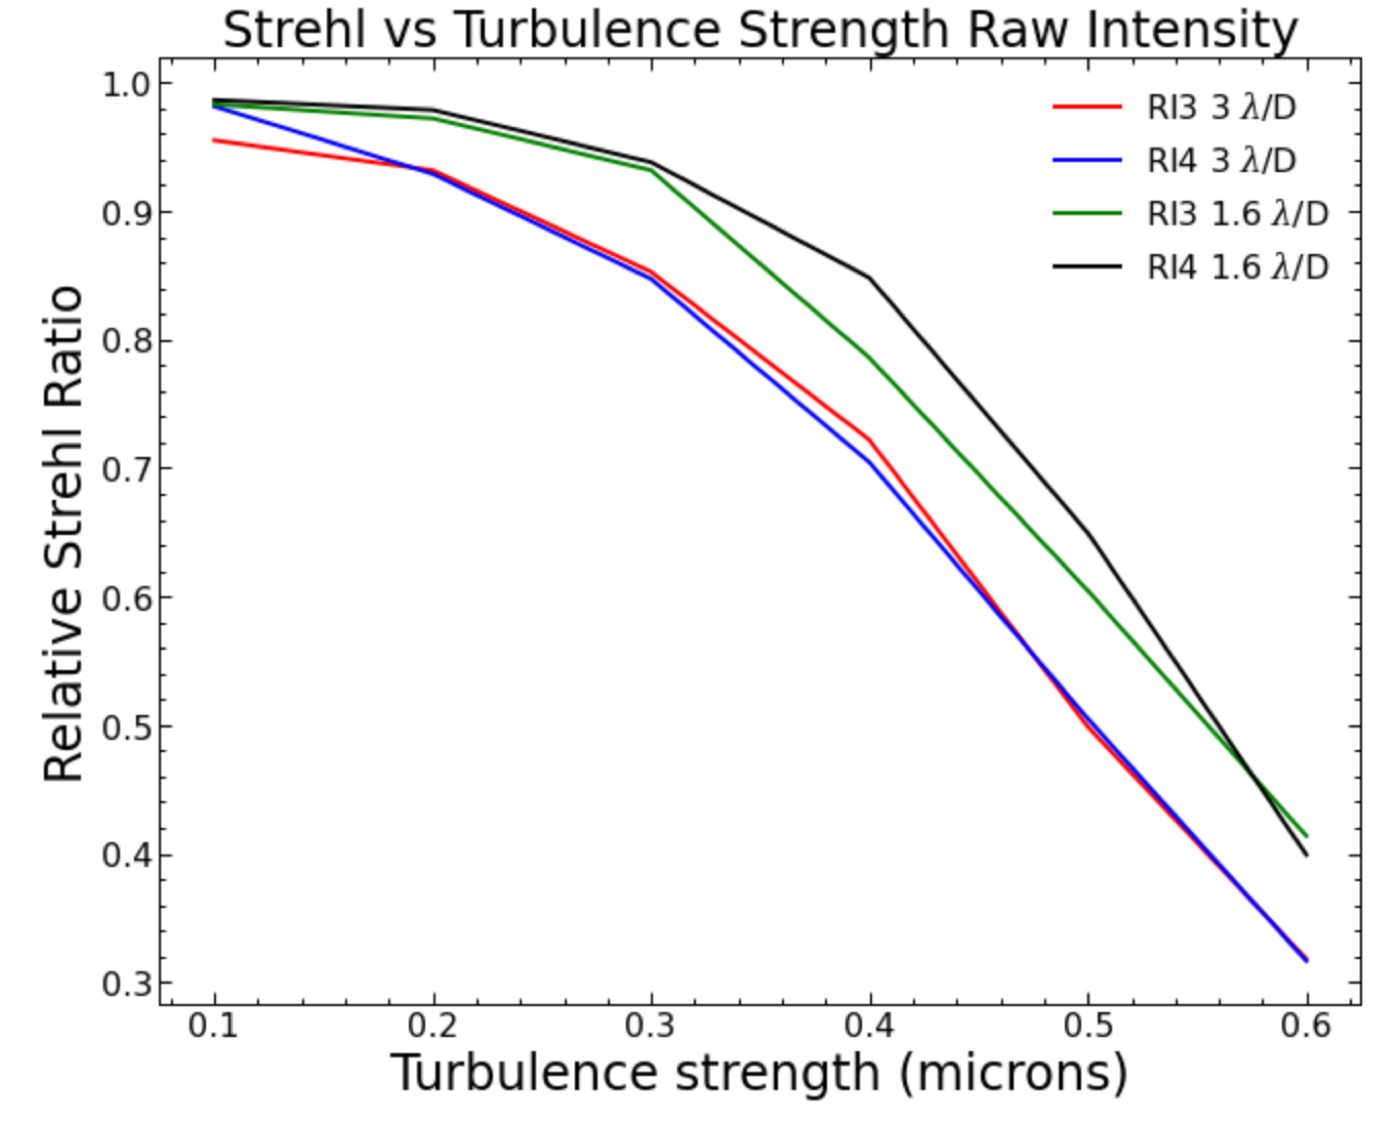
\includegraphics[width=0.8\textwidth]{Chapter Materials/Chapter Five Materials/RawIntensityStrehlVSTurb.png}
    \caption{Relative Strehl ratio versus turbulence strength for the 3PWFS and 4PWFS using the Raw Intensity signal processing method. The performance of each wavefront sensor at both 3.25 $\lambda/D$ and 1.6 $\lambda/D$ are comparable. A slight increase in performance is seen when moving to lower modulation. }
    \label{fig:RI}
\end{figure}

The performance of the PWFS using the Slopes Maps calculation was more uniform. The relative Strehl ratio calculated for the 3PWFS and 4PWFS at 3.25 $\lambda/D$ and 1.6 $\lambda/D$ are comparable. Figure \ref{fig:SM} plots the relative Strehl ratio as a function of turbulence strength for the PWFS using the Slopes Maps calculation.

\begin{figure}
    \centering
    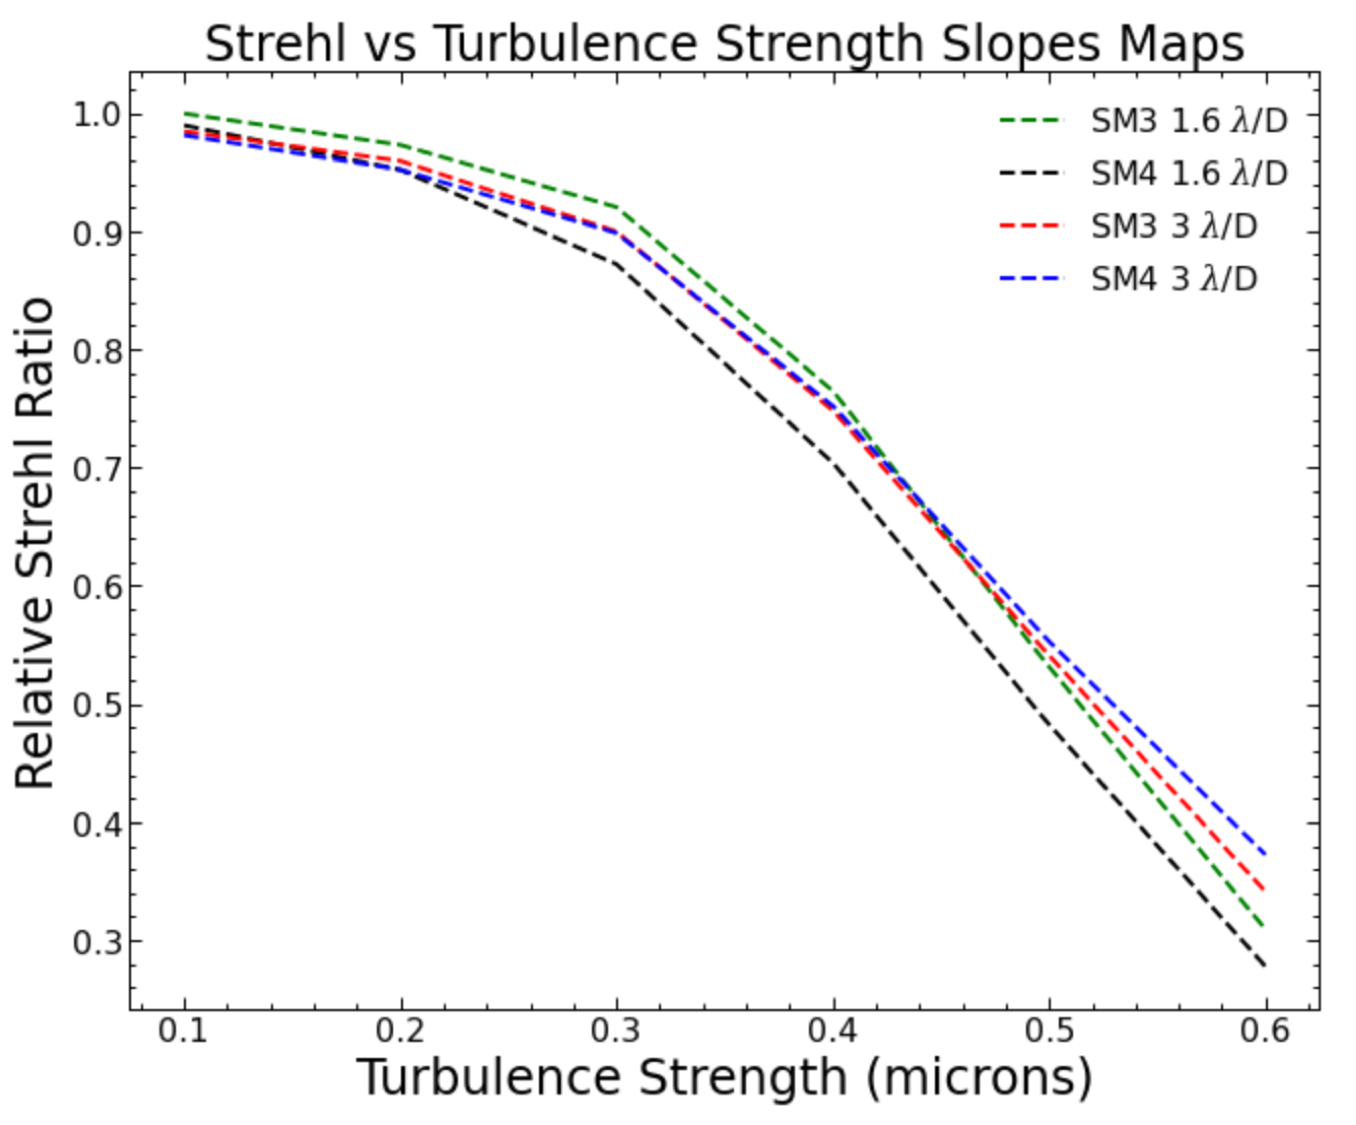
\includegraphics[width=0.8\textwidth]{Chapter Materials/Chapter Five Materials/SlopesMapsStrehlVsTurb.png}
    \caption{Relative Strehl ratio versus turbulence strength for the 3PWFS and 4PWFS using the Slopes Maps signal processing method. The performance of each wavefront sensor across all modulations radii and turbulence strengths are comparable.}
    \label{fig:SM}
\end{figure}

Figure \ref{fig:All} plots all of the results from both the RI and SM trials onto a single plot. This plot shows that the best performance was obtained by the 4PWFS using RI at 1.6 $\lambda /D$ modulation. Referring back to the plot in Figure \ref{fig:gains}, we can see that this trial also used the highest modal gains. This suggests that this increase in performance for the 4PWFS is not real, and that the modal gains for the other trials were not properly optimized and that increasing the modal gains could have increased performance.


\begin{figure}
    \centering
    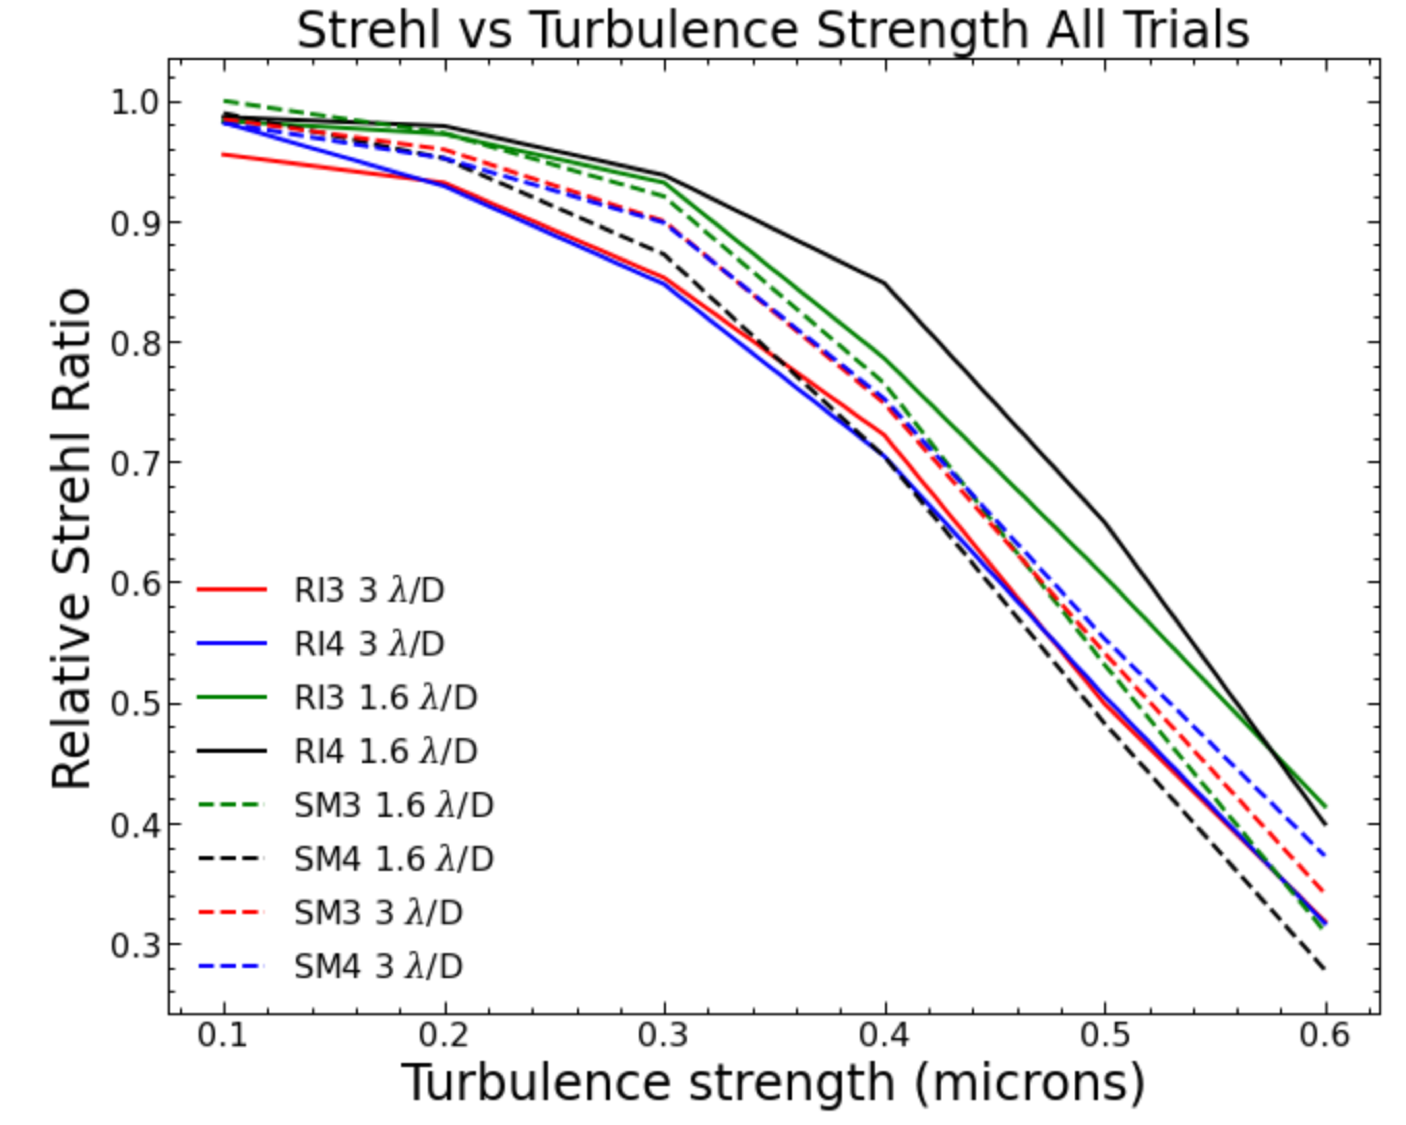
\includegraphics[width=0.8\textwidth]{Chapter Materials/Chapter Five Materials/AllTrialsStrehlVSTurb.png}
    \caption{Summary of all results. Best performance was achieved using the 4PWFS at 1.6 $\lambda/D$ modulation using RI. However, this trial had the highest modal gains set, implying that this performance is not real, but that the modal gain for the other trials was set too low.}
    \label{fig:All}
\end{figure}

\section{Discussion}
In the current configuration a 3PWFS and 4PWFS were integrated into CACTI for a performance test. Both PWFS were designed with refractive pyramid optics, and had similar sampling across the pyramid pupils. Effort was put into minimizing the differences between each PWFS. Non-common path error was minimized by ensuring each pyramid optic had the same PSF on the tip. Two different signal handling methods were employed on CACTI to process the PWFS signals. It was found that the Slopes Maps method was highly sensitive to changes in alignment, requiring new calibrations every time the CACTI system was started up. The CACTI testbed uses a circle fitter algorithm to determine where the pupils are cropped out to perform the Slopes calculation. It was found that a sub-pixel shift of the pupil, with respect to the position at calibration, was enough misalignment to cause the calibration to become inoperable and the loop to diverge. The Raw Intensity method was found to be less sensitive, and a calibration taken days in advanced was able to still be used to close the AO loop.

A concern for the 3PWFS is that the wavefront is sampled with three points instead of four, and thus potentially has a larger null space than the 4PWFS. This would mean fewer modes are sensed, and the accuracy of the wavefront sensing is reduced. On the CACTI testbed, we found that the difference in sampling did not impact system performance, or effect the number of modes the AO was able to close on. A summary of the number of basis set modes that were used to close loop for each PWFS and signal processing method can be found in Table \ref{tab:Modestable}. The number of modes used is determined by CACAO during calibration. 

\begin{table}
	\begin{center}
		\begin{tabular}{ | l|l|l | l| }
			\hline
			\textbf{PWFS}& \textbf{Signal Processing} &\textbf{Modulation radius} &\textbf{$\#$ of Modes}\\ \hline
             3PWFS & Raw Intensity & 3.25 $\lambda/D$ & 515\\ \hline
             3PWFS & Raw Intensity & 1.6 $\lambda/D$ & 507 \\ \hline
             3PWFS & Slopes Maps &  3.25 $\lambda/D$ &493 \\ \hline
             3PWFS & Slopes Maps &  1.6 $\lambda/D$ & 496\\ \hline
             4PWFS & Raw Intensity & 3.25 $\lambda/D$ & 516\\ \hline
             4PWFS & Raw Intensity & 1.6 $\lambda/D$ & 513\\ \hline
             4PWFS & Slopes Maps &  3.25 $\lambda/D$ & 497 \\ \hline
             4PWFS & Slopes Maps &  1.6 $\lambda/D$ & 502\\ \hline
			\end{tabular}
		\end{center}
	\caption{Number of basis set modes used for the AO closed loop for each PWFS and signal processing method.}
	\label{tab:Modestable}
\end{table}

The performance of each wavefront sensor on the CACTI testbed was determined to be similar for each modulation radius and turbulence strength. The difference in performance for the Raw Intensity method for the 1.6 $\lambda/D$ and 3.25 $\lambda/D$ modulation cases was on average 0.069 Strehl for the 3PWFS, and 0.086 Strehl for the 4PWFS. It has been shown \cite{guyon2005}$^,$ \cite{verinaud2004nature} that the sensitivity of the PWFS is increased by decreasing the radius of modulation. We cannot definitively conclude that the increase in performance of the 1.6 $\lambda/D$ modulation case was due to the increase in PWFS sensitivity due to systematic errors such as misalignment, imperfect calibrations, or imperfect selection of modal gains. The performance of each wavefront sensor was maximized when the modal gains were tuned. Modal gain tuning is therefore a necessary step to optimize the correction of an ExAO system. Nothing in our experiments indicated that with proper gain tuning the performances of the 3PWFS and 4PWFS should be different.

% The power of low order modes of the turbulence screens used by CACTI are filtered so that the full stroke of the DM is not used. \jrmcom{This isn't quite right.  The power at low spatial frequencies is lower than it would be in unfiltered Kolmogorov turb, but it is still higher than at higher spatial frequencies.  That is, the filter does not set it to 0.} Most of the power in the spatial frequencies of the turbulence screen power spectrum are mid to high spatial frequencies. \jrmcom{So this statement might be too big:}Our results suggest that modulating decreases sensitivity across all spatial frequencies, and that the AO system should be run at as small of a modulation radius as possible. 
